\chapter{Deep Learning and Neural Networks}

In the Machine Learning framework the so-called feature learning represents a class of methods whose goal is to create computing systems able to solve specific tasks, like detecting particular behaviours of structures or classifying a particular object, starting from the raw data.

Deep learning methods are a part of this family and have been applied in many fields, such as audio recognition and computer vision. Often this methods makes use of Artificial Neural Networks. Deep Learning is in fact usually referred to the use of Artificial Neural Networks with a multiple layer structure, from which the adjective 'deep' derives, as we will describe in the following.

\section{Artificial Neural Networks}

Artificial Neural Networks (ANNs in the following) are also denoted as biological-inspired networks; this denominations derives from their structure, which is inspired from  the brain of the animals. As for a natural brain, where each neuron communicates with others through the synapses, ANN are computing systems based on a series of units, called artificial neurons, connected among themselves. 

The simplest model used to represent an artificial neuron, capable of simple learning tasks, is the perceptron, invented in 1958 by Frank Rosenblatt, which, given a series of binary input values $\bar{x}=\{x_1,\dots, x_n\}$ returns a single binary output value $f(\bar{x}, \alpha)$, where $\alpha$ are the internal parameters of the perceptron. 

The internal structure on the perceptron, represented in \figref{fig:perceptron}, is composed of a series of real-valued weights $\bar{w}=\{w_1,\dots,w_n\}$, a bias value $b$ and a threshold $\delta$. These parameters are used by the decision function $f$ to estimate the output value:

\begin{equation}
f(\bar{x},\alpha) = 
\begin{cases}
0\qquad\text{if}\quad\sum_{i=1}^N x_iw_i \leq \delta \\
1\qquad\text{if}\quad\sum_{i=1}^N x_iw_i > \delta \\
\end{cases}
\end{equation}

\begin{figure}[h]
    \centering
\includestandalone[height=6cm, width=\textwidth]{images/networks/perceptron}
\caption{Internal structure of a perceptron.}
    \label{fig:perceptron}
\end{figure}

\section{Neural Network architectures}

The perceptron model is unable to solve the complex tasks that are common nowadays in the Deep Learning field. In order to solve this tasks more complex models for the artificial neurons are used but, more importantly, the neurons are combined in order to create an Artificial Neural Network or ANN.

In most common applications the neurons are organized in consecutive layers.
In this structure each layer receives a series of values as input and produces an output which is used, with some manipulations, as input for the subsequent layer. The layers are usually denominated as following:
\begin{itemize}
    \item \textbf{Input Layer}: the first layer of the ANN, its input values are externally provided, i.e. an image for a classification task
    \item \textbf{Output Layer}: the last layer of the ANN, its output value is used as the prediction for the type of task the network is trying to solve
    \item \textbf{Hidden Layers}: all the intermediate layers of the network  
\end{itemize}

A first distinction in the structure of an ANN can be done between fully and partially connected ones. The former ones use as input of each neuron of a layer the output of all the neurons of the previous layer, the latter instead uses only a subset of those. A graphical representation of this difference is displayed in \figref{fig:full_part_ANN}.

\begin{figure}[h]
    \centering
    \begin{minipage}[c]{0.49\linewidth}
        \vspace{0pt}
        \centering
        \subfloat[Example of fully connected ANN structure]{
        \includestandalone[height=5cm, width=\textwidth]{images/networks/full_net}
            \label{fig:full_ANN}
        }
    \end{minipage}%
    \hfill%
    \begin{minipage}[c]{0.49\linewidth}
        \vspace{0pt}
        \centering
        \subfloat[Example of partially connected ANN structure]{
\includestandalone[height=5cm, width=\textwidth]{images/networks/partial_net}            \label{fig:part_ANN}
        }
    \end{minipage}%
    \caption{Graphical comparison of the architecture of a fully connected ANN and a partially connected one. The circles represent artificial neuron while grey lines indicate the connection between them.}
    \label{fig:full_part_ANN}
\end{figure}

An important aspect to highlight is that, due to the layered structure of the ANNs, we can disengage ourself from mathematically represent each single artificial neuron of the network and treat each  layer as a single mathematical object. \\
Given an ANN composed of $N_L$ consecutive layers, where the $i$-th layer is denoted with $L_i$, we can represent the output of a layer as a function:
\begin{equation}
    f_L^i (\bar{x_i})=a_i \left( \tilde{f}(\bar{x_i}, \boldsymbol{w}_i) + \bar{b}_i \right) 
    \label{eq:layer_math}
\end{equation}

where $\bar{x}_i$ is the input of the layer, $\boldsymbol{w}_i$ is a matrix of free parameters, called weights and $\bar{b}_i$ is a bias vector also composed of free parameters. The $\tilde{f}$ function is the key mathematical operation of the layer, whose choice leads to very different types of layers, which are then used to create specific types of ANNs, as described in \secref{ANN_type}. The $a_i$ function is the so-called activation function, whose choice plays a crucial role is the ability of the network to solve a specific task. Some of the possible choices for this function are reported in \secref{activations}.
This representation then allows us to represent an artificial neural network, composed of $N_L$ layers, as a set $\mathcal{F}_{N_L}$:
\begin{equation}
\mathcal{F}_{N_L} = \left\{ f_N(\bar{x}), \boldsymbol{w}, \bar{b}\right\}
\end{equation}

where $\boldsymbol{w} = \{\boldsymbol{w}_1 \dots \boldsymbol{w}_{N_L}\}$ and 
$ \bar{b} = \{ \bar{b}_1 \dots  \bar{b}_{N_L}\}$ are respectively the set of all the layer weight and biases and the $f_N(\bar{x})$ is the composition of the $f_L^i(\bar{x_i})$
functions:
\begin{equation}
    f_N(\bar{x}) = f_L^{N_L} \circ f_L^{N_L-1}\circ\dots\circ f_L^2\circ f_L^1 (\bar{x}) 
\end{equation}

Now that the structure of an ANN has been defined the most important question is how to find the best $\boldsymbol{w}$ and $\bar{b}$ parameters for a specific task.
Given a particular network structure and an input dataset $\mathcal{D}$, the best parameters  are estimated through a procedure called "training". In this procedure we define a loss function, which estimates how well the network is currently solving the task, and then utilize an algorithm which minimizes it by modifying the free parametes of the network. This steps are further explained respectively in \secref{lossfunction}
and \secref{weightoptimization}.

\subsection{Activation functions}\label{activations}

As shown in \forref{eq:layer_math} an ANN layer can be mathematically represented as:
\begin{equation}
    f_L^i (\bar{x_i})=a_i \left( \tilde{f}(\bar{x_i}, \boldsymbol{w}_i) + \bar{b}_i \right) 
    \label{eq:layer_math}
\end{equation}

where $a_i$ is the so-called activation function. The choice of this function plays a crucial role in determining both the capability of the network of solving the assigned task and also  the time needed for it to be able to solve it efficiently, namely different activation function may need a longer training than others. The choice of this function depends on various factors but the most important surely are the position of the layer inside the network and the specific task we are trying to solve.

The position inside the network is relevant since the hidden layers of the network are usually built using activation functions with output values in $\mathbb{R}$ or $\mathbb{R}^+$ while for the output layers activation functions with values in $[0,1]$ or $[-1,1]$ are preferred in order to interpret the results as a probability.
The specific task, on the other hand, mainly influences the activation function of the output layer since different tasks often requires a different output structure.
In the following a list of the most commonly used functions is presented.

\begin{figure}[!h]
\begin{minipage}{0.45\textwidth}
    \centering
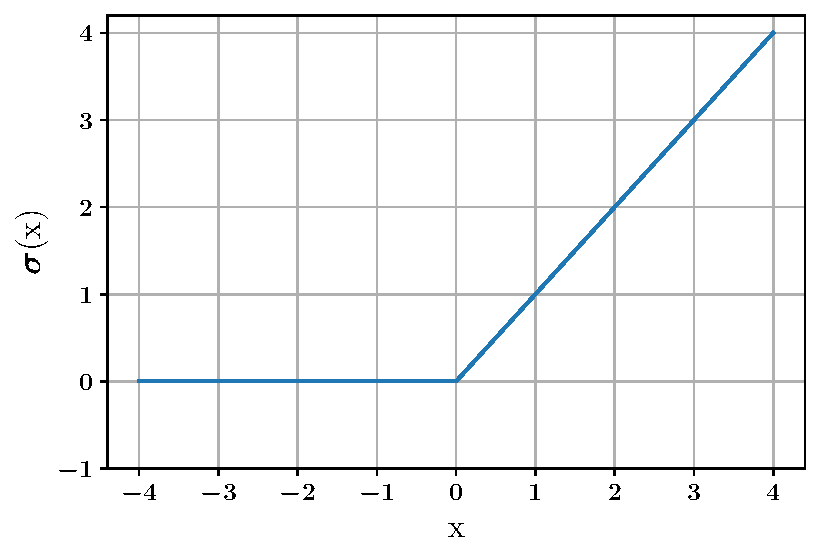
\includegraphics[width=\textwidth]{images/networks/act_relu.pdf}
\caption{ReLU activation function}
    \label{fig:act_relu}
\end{minipage}
\hfill
\begin{minipage}{0.5\textwidth}
    \textbf{Rectified Linear Unit (ReLU)}
   \begin{align}
        a(x) &=
        \begin{cases}
        x   & \text{if } x > 0 \\
        0  & \text{if } x \leq 0 
  \end{cases}
\end{align}
The ReLU is a continuous function with a point of non differentiability in 0. Despite being non differentiable this function is still implemented, mostly in the hidden layers of a network, due to its fast computation time. 
\end{minipage}
\end{figure}

\begin{figure}[!h]
\begin{minipage}{0.45\textwidth}
    \centering
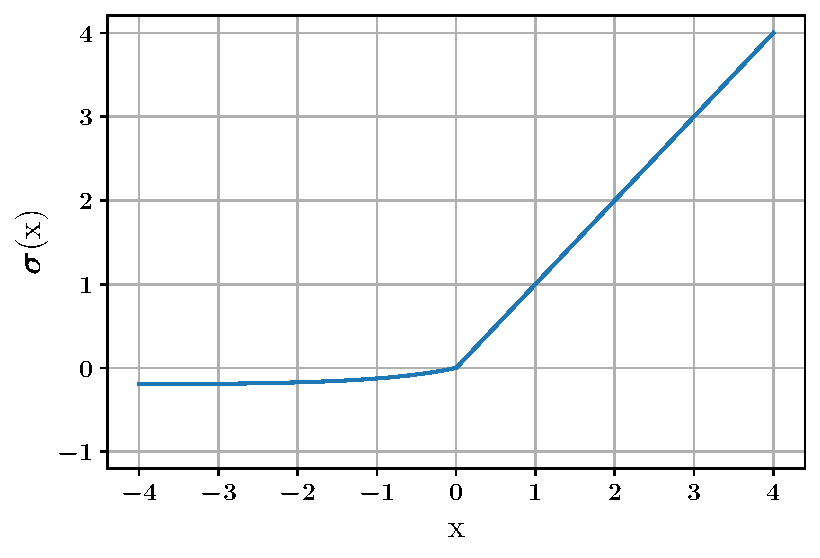
\includegraphics[width=\textwidth]{images/networks/act_elu.pdf}
\caption{ELU activation function}
    \label{fig:elu}
\end{minipage}
\hfill
\begin{minipage}{0.5\textwidth}
    \textbf{Exponential Linear Unit (ELU)}
   \begin{align}
        a(x) &= 
        \begin{cases}
        \alpha \left(e^x -1\right)  & \text{if } x \leq 0 \\
        x  & \text{if } x > 0 
  \end{cases}
\end{align}
The ELU activation functions is an improvement over the ReLU. In this case the negative values have an actual activation instead of being set to zero which may help the estimation of the network parameters. The drawback of choosing this function in an increase in the computational cost since an exponential operation is included. 
\end{minipage}
\end{figure}

\begin{figure}[!h]
\begin{minipage}{0.45\textwidth}
    \centering
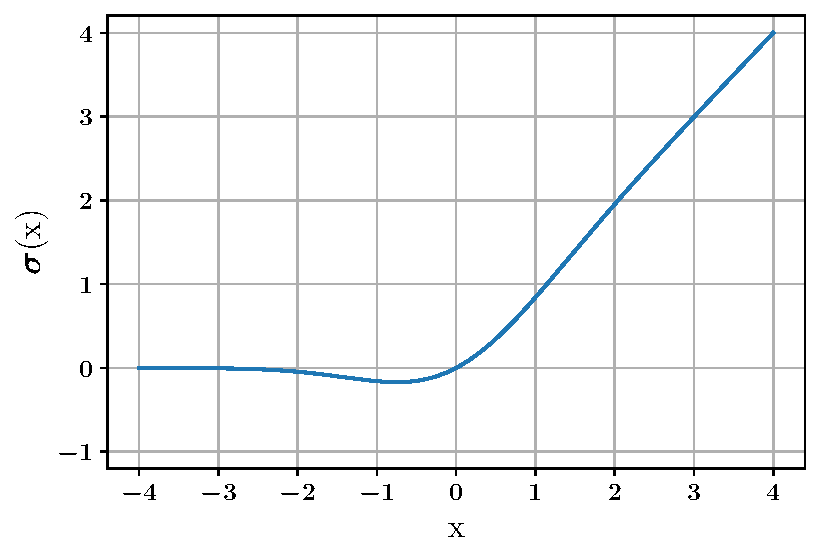
\includegraphics[width=\textwidth]{images/networks/act_gelu.pdf}
\caption{GELU activation function}
    \label{fig:gelu}
\end{minipage}
\hfill
\begin{minipage}{0.5\textwidth}
    \textbf{Gaussian Error Linear Unit (GELU)}
   \begin{equation}
       a(x) = \frac{1}{2} x \left( 1+\text{erf} \left( \frac{x}{\sqrt{2}}\right)\right)
   \end{equation}
   This is one of the newest activation functions. It was implemented in some of the most recent Deep Learining application proving to be one of the best activations in the Natural Language Processing field. 
\end{minipage}
\end{figure}

\begin{figure}[!h]
\begin{minipage}{0.45\textwidth}

    \centering
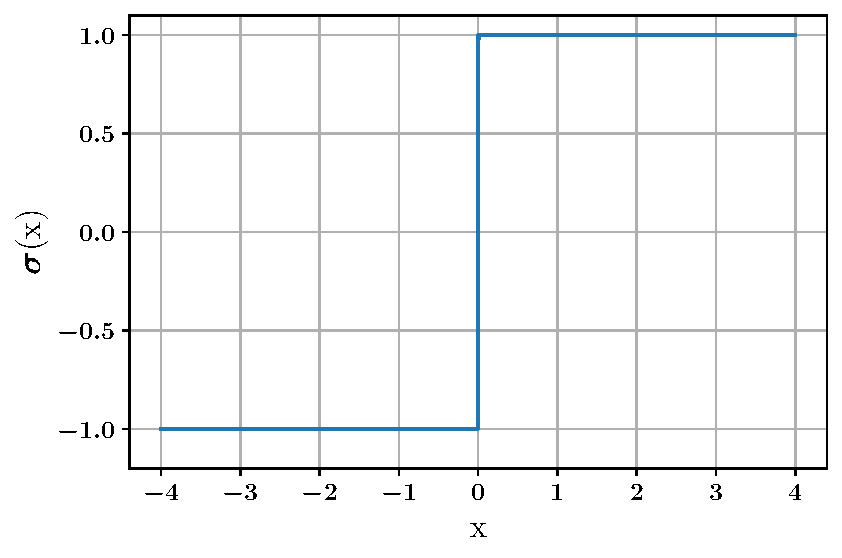
\includegraphics[width=\textwidth]{images/networks/act_step.pdf}
\caption{Step activation function}
    \label{fig:act_step}
\end{minipage}
\hfill
\begin{minipage}{0.5\textwidth}
    \textbf{Binary step}
      \begin{align}
        a(x) &=
        \begin{cases}
        1   & \text{if } x \geq 0 \\
        -1  & \text{if } x < 0 
  \end{cases}
\end{align}
Neurons using this function are also called linear threshold units(LTU). This type of neurons can be used for solving simple tasks but is not able to solve complex tasks like multiclass classifications or image recognitions.
\end{minipage}
    \end{figure}

\begin{figure}[!h]
\begin{minipage}{0.45\textwidth}

    \centering
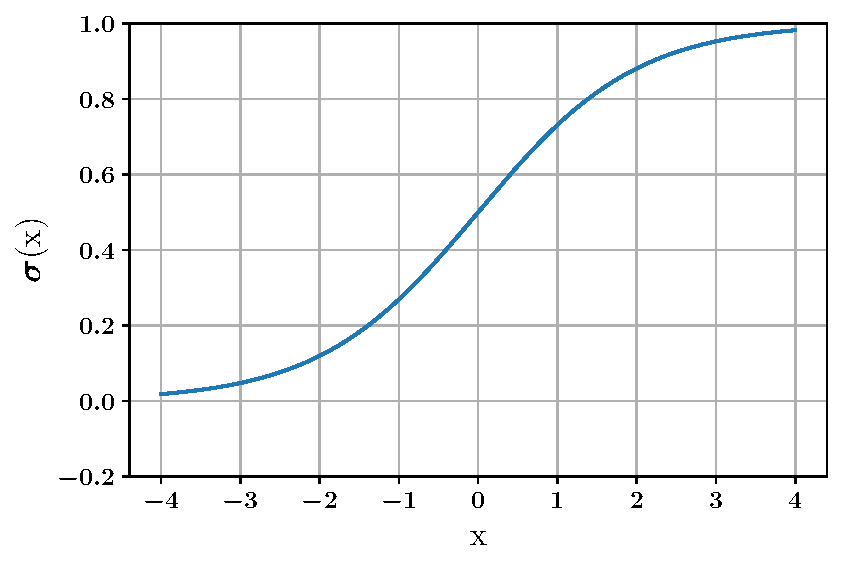
\includegraphics[width=\textwidth]{images/networks/act_sig.pdf}
\caption{Sigmoid activation function}
    \label{fig:act_sig}
\end{minipage}
\hfill
\begin{minipage}{0.5\textwidth}
    \textbf{Sigmoid} or \textbf{Soft step}
   \begin{equation}
       a(x) =\frac{1}{1+e^{-x}}
   \end{equation}
   The sigmoid functions provides an output value in $[0,1]$ and is differentiable in every point. This properties makes it one of the most used activation functions for the last layer of an ANN.
\end{minipage}
    \end{figure}


\begin{figure}[!h]
\begin{minipage}{0.45\textwidth}
    \centering
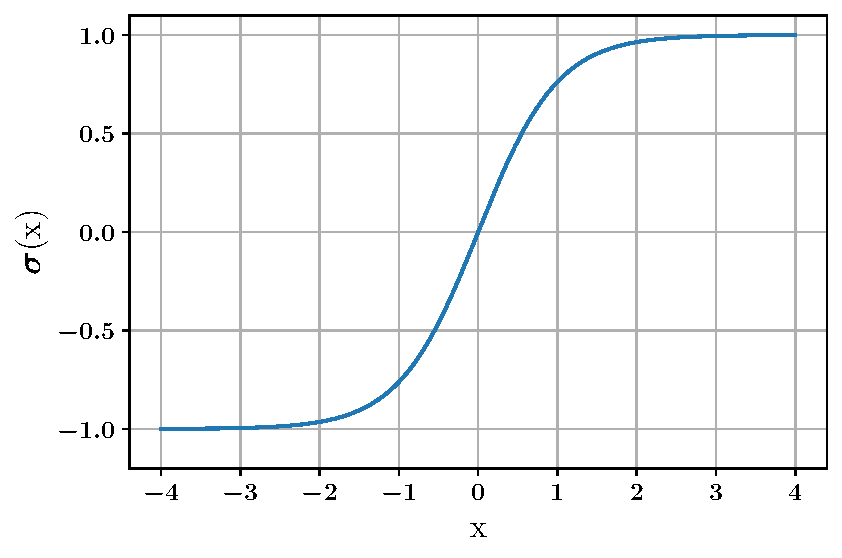
\includegraphics[width=\textwidth]{images/networks/act_tanh.pdf}
\caption{Hyperbolic tangent activation function}
    \label{fig:act_tanh}
\end{minipage}
\hfill
\begin{minipage}{0.5\textwidth}
    \textbf{Hyperbolic tangent}
   \begin{equation}
       a(x) =\frac{e^x-e^{-x}}{e^x+e^{-x}}
   \end{equation}
The hyperbolic tangent has similar properties to the sigmoid function. Its output is however in $[-1,1]$ which may speed up convergence in same applications.
\end{minipage}
\end{figure}

 

\section{Types of Artificial Neural Network and layer structure}
\label{ANN_type}

As described in the previous section, a layer of an ANN can be represented by its key mathematical operation. In the most common applications this operation is a function depending of the input vector of the layer and of a series of free parameters called weights.

The choice of this operation is of fundamental importance since the whole behaviour of an ANN depends on it. More specifically the choice of this operation determines the type of the layer and, consequently, the type of ANN we are creating. 

There are many possible choices and architectures but, for this work, we will focus on the main two type of Artificial Neural Networks and their type of layers: Dense Neural Networks and Convolutional Neural Networks, respectively described in \secref{dnn} and \secref{cnn}.
It is important to highlight that, despite being described separately, this two architectures can be combined together, as we will see in the following chapters, in order to create a better predictor.

\subsection{Dense Neural Networks}\label{dnn}

Dense neural networks, also known as DNNs, are Artificial Neural Networks with many fully connected hidden layers between the input and output ones, this result in a high number of connections between the units from which the 'dense' adjective derives.

Following directly from this denominations the fully connected layers that compose a Dense Neural Network are called Dense Layers.
A dense layer, whose decision function will denoted with $f_D$, is characterized by the dot product $\cdot$ as its key mathematical operation, using the notation previously introduced it can then be represented as:
\begin{equation}
    f_D (\bar{x})=a_i \left( \bar{x} \cdot \boldsymbol{w} + \bar{b}_i \right) 
    \label{eq:layer_dense}
\end{equation}

Depending on the structure of the input vector $\bar{x}$ and on the weight tensor $\boldsymbol{w}$ the dot product represent a different mathematical operation, specifically:
\begin{itemize}
    \item if both $\bar{x}$ and $\boldsymbol{w}$ are 1-dimensional vectors the dot product corresponds to the inner product of the two
    \item if both $\bar{x}$ and $\boldsymbol{w}$ are 2-dimensional, namely they are matrices, the dot product corresponds to the matrix-matrix multiplication of the two
     \item if either one is a scalar value then the dot product corresponds to a simple multiplication where the scalar is used as a factor
     \item if $\bar{x}$ and $\boldsymbol{w}$ respectively are an N-dimension and M-dimension tensor the dot product becomes a sum product over their last dimensions
\end{itemize}

In \figref{fig:dnn_example} an illustration of the structure of a simple DNN is reported. DNNs are commonly used to solve many tasks but the field in which they are mostly implemented is the classification, due to their ability of easily understanding both linear and non-linear patterns in a multi-variate analysis.


\begin{figure}
    \centering
\includestandalone[width=0.8\textwidth]{images/networks/DNN}
    \caption{Example of the structure of a Dense Neural Network. The neurons of each layer are represented by circles while the grey lines represent connections between them.}
    \label{fig:dnn_example}
\end{figure}

One of the main drawbacks of the usage of DNNs is however the number of free parameters. Dense layers are in fact characterized by an high number of weights and, due to the fully connected structure of the network, the total number of parameters grows really fast with each additional layer. 
A too high number of parameters may lead to two main issues. The first problem one may encounter is the inability of the network to correctly estimate the optimal parameters, resulting in its inability of giving correct prediction. The second possible issue is the so-called over-fitting problem, namely the network adapts too well to the data on which its train is performed, but again gives completely wrong prediction when tested on other data. A brief explanation of this issue is discussed in \secref{fit_over_under}.
To avoid this issues the number of free parameters can be controlled, working on two factors: the shape of the input vector, which depends on the specific tasks but can sometimes be modified or reduced using techniques such as the PCA, and the number of neurons in each layer, which can be selected in order to reach the best compromise between performances and model complexity.

\subsection{Convolutional Neural Networks}\label{cnn}

Another type on ANN is the so-called Convolutional Neural Network, also known as CNN. As the name suggests the key mathematical operation in the layers of this type of network is the convolution, this layers are therefore called Convolutional Layers, from which the CNN name derives.

The key elements of a convolutional layers are the so-called filters. The output of a convolutional layer is fact computed as the resulting vector of the discrete convolution of the input values with each filter. 

\begin{wrapfigure}{r}{0.5\textwidth}
    \centering
  \includestandalone[width=0.5\textwidth]{images/networks/CNN}
    \caption{Example of the combination of a convolutional layer with one 1 dimensional filter and a max pooling layer performing.  }
    \label{fig:cnn_tot}
\end{wrapfigure}
The filters of a CNN have the same role of the weight tensor of a DNN and are in fact the free parameters of the network, whose optimization is performed during the training. In \figref{fig:cnn_filter} an example of the result of the application of a filter to a 2-dimensional input is shown.

In most of the common implementations however CNNs are not composed of only convolutional layers but are made of an alternation of convolutional and pooling layers, where the latter is used to  perform a non-linear down-sampling on the output of a convolutional layer. An example of the combination of these two layers is shown in \figref{fig:cnn_tot}


More specifically a pooling layer divides its input in a series of region called "pools" and applies a function to each one.
The resulting value from all pools is then combined and used as the output of the layer.

Many choices for both the size of the pools and the function to apply are possible however one of the most common implementation is a max-pooling layer with a 2x2 pool size, namely a layer that divides the input in 2x2 regions and takes the highest value from each of them. A example of the application of this type of layer is shown in \figref{fig:cnn_pool} 

\begin{figure}[h]
    \centering
      \includestandalone[height=6cm, width=\textwidth]{images/networks/cnn_filter}
    \caption{Example of the application of a filter over a 2 dimensional input. The resulting matrix is computed as the discrete convolution of the input with the filter values.}
    \label{fig:cnn_filter}
\end{figure}

\begin{figure}[h]
    \centering
     \includestandalone[height=5cm, width=0.85\textwidth]{images/networks/cnn_pool}
    \caption{Example of the application of the max pooling operation over a 2 dimensional input, with 2x2 pool size. The resulting matrix is computed as the maximum value of each 2x2 pool.}
    \label{fig:cnn_pool}
\end{figure}


%\begin{wrapfigure}{r}{0.5\textwidth}
%    \centering
%  \includestandalone[height=7cm, width=0.6\textwidth]{images/networks/CNN}
%    \caption{cnn }
%    \label{fig:cnn_tot}
%\end{wrapfigure}


\section{Loss functions} \label{lossfunction}

After the choice of the ANN type and its internal structure the next step is to choose the so-called loss function, also known as risk or cost function. The role of the loss function is to quantify how well the predicting power of the network is and its choice plays a crucial role in the learning procedure.

In most Deep Learning application the role of the learning algorithm is in fact to estimate the best set of parameters that are able to minimize the value of the loss function over a set of given input values. The choice of this function is therefore really important since it may greatly influence the final ability of the model of producing correct predictions.

As for the activation functions many choices of the loss function are possible. In the following part we present a brief list of the ones implemented in the most common applications:
\begin{itemize}
    \item \textbf{Mean Squared Error} or \textbf{L2 Loss}:\\
    This loss computes the average of the squared distance between the correct label associated to a sample, $y_{i,T}$ and the predicted one, $y_{i,P}$:
    \begin{equation}
        L_{MSE}= \frac{1}{N}\sum_{i=1}^N \left(y_{i,T}-y_{i,P}\right)^2
    \end{equation}
    This function is mostly implemented in regression tasks and is characterized by the heavy penalization imposed on predicted values very distant from their correct label.
    \item \textbf{Mean Absolute Error} or \textbf{L1 Loss}:\\
    This loss computes the average of the absolute distance between the correct label associated to a sample, $y_{i,T}$ and the predicted one, $y_{i,P}$:
    \begin{equation}
        L_{MAE}= \frac{1}{N}\sum_{i=1}^N \left|y_{i,T}-y_{i,P}\right|
    \end{equation}
    Similarly to the L2 loss also the L1 is used in regression tasks but it penalizes more many small deviation from the correct label than few very distant ones. Respect to the L2 loss the L1 has the drawback of needing more complex tools for the computations of the gradient. 
\item \textbf{Hinge Loss}:\\
    The hinge loss is mostly famous for its implementation in Support Vector Machines (SVMs). As for the previous losses the Hinge one is a function of the true, $y_{i,T}$ and  predicted label, $y_{i,P}$ but with the constraint of them being either $\pm 1$:
    \begin{equation}
        L_{H}= \sum_{i=1}^N \max\left( 1-y_{i,T}*y_{i,P},0\right)
    \end{equation}
\item \textbf{Binary Cross Entropy Loss}:\\
    This function is the standard loss implemented for the binary classification tasks. It is computed using the true label associated to the i-th sample, requested to be a binary value, $y_{i,T}\in{0,1}$ and the probability $p_{i}$ of it being associated to the class indicated with $y_{T}=1$. With this notation the loss function is written as:
    \begin{equation}
        L_{BCE}= -\sum_{i=1}^N\left[ y_{i,T}\log(p_i)+
        \left(1- y_{i,T}\right)\log(1-p_i)\right]
    \end{equation}
    This loss function is characterized by heavy penalization of confident but wrong predictions. 
\item \textbf{Categorical Cross Entropy Loss}:\\
    This loss function is the natural generalization of the previous one. As such it is the standard function implemented in multi-class classification tasks. Considering a classification tasks with $M>2$ classes, we associate to i-th sample a set of probabilities $p_{i,c}$, which represent its probability of belonging to the class $c$ and a set of binary values $y_{i,c}$ whose value is 1 only for the correct class the sample belong to. Using this notation the loss function is defined as:
    \begin{equation}
        L_{CCE} = -\sum{i=1}^N \sum_{c=1}=M  \left[
        y_{i,c}\log(p_{i,c}) + (1-y_{i,c})\log(1-p_{i,c})
        \right]
    \end{equation}
\end{itemize}


\subsection{Overfitting and underfitting recognition} \label{fit_over_under}

Aside from being the quantity used to estimate the optimal parameters of a predictor the loss function is also used to monitor the performance in search of over and under fitting bahaviour during the learning procedure. 
This issues can be observed dividing the given dataset $\mathcal{D}$ in two parts: a training dataset $\mathcal{D_{Tr}}$ and a test dataset $\mathcal{D_{Te}}$\footnote{In many applications the dataset is not split in two but rather three subsets, namely the training $\mathcal{D_{Tr}}$, validation $\mathcal{D_{V}}$ and test $\mathcal{D_{Te}}$ set. In this case the validation set is used to monitor the eventual presence of over and under fitting while the test set is used to evaluate the final performance of the model. As we will see in the following chapters this strategy of division is also the one implemented in this work.}. As the name suggests the training dataset is used to train the predictor while the test set is used to verify the effective performance after the learning.

The overfitting issue is observable in cases where the prediction model adapts too well to the training set, failing to give good predictions on the test set. This issue is common in cases where the complexity of the model is too high compared to the size or structure of the given dataset or when the training is performed for too long. Possible ways to resolve the overfitting issue are using a simplified model or using some optimization techniques, such as the regularization and dropout, described in \secref{opt_tec}.
The opposite of the overfitting is the so-called under fitting. This issue arises whenever there is still room for improving the model prediction capability. Possible ways to resolve this issue is the introduction of a more complex model or just increasing the training time.

In order to visualize this two issues, lets for example consider the simple task of performing a polynomial fit over a given distribution, as shown in  \figref{fig:overunderfit}. The data samples in this figure have been generated from a second degree polynomial distribution plus some gaussian noise and divided in training, over which the fit is performed, and test samples. The distribution is then fitted with a first, second and 10-th degree polynomial and the MSE Loss, introduced before, is computed. As we can see the second order polynomial fit has similar training and the fit well represents both the distribution. On the other hand the first order fit instead has a very high training and test error which is a clear sign of the underfitting issue. Finally the 10-th order polynomial fit presents a very low training error and an high test error which indicates that the estimated distriubution is overfitted on the training set but does not represent effectively the full distribution.

\begin{figure}[h]
    \centering
    \begin{minipage}[c]{0.49\linewidth}
        \vspace{0pt}
        \centering
        \subfloat[1st order polynomial fit]{
        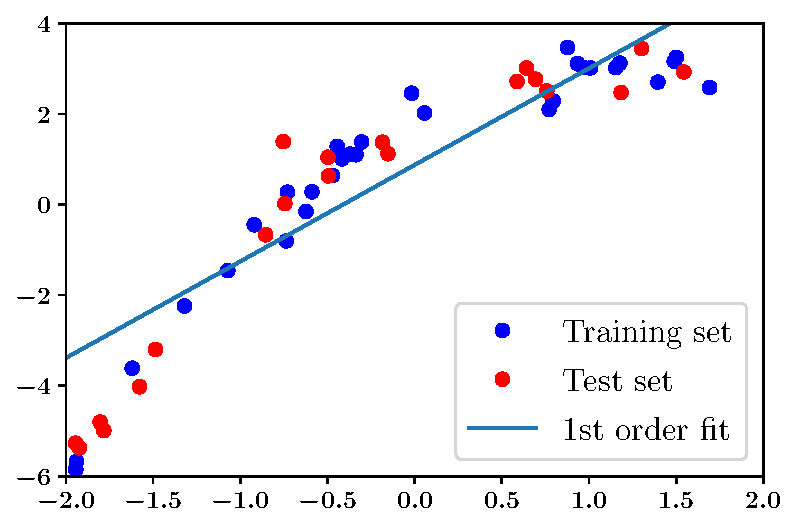
\includegraphics[width=\textwidth]{images/networks/over_under_fit_p1.pdf}
            \label{fig:p1_fit}
        }
    \end{minipage}%
    \hfill%
    \begin{minipage}[c]{0.49\linewidth}
        \vspace{0pt}
        \centering
        \subfloat[2nd order polynomial fit]{
        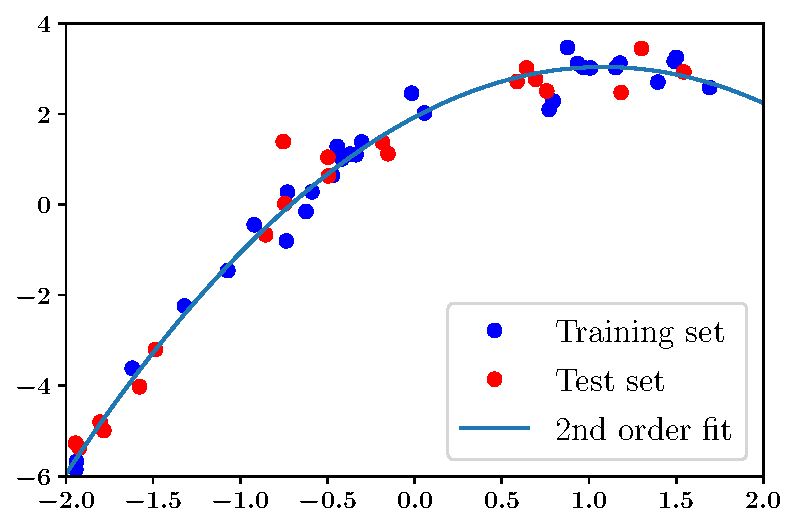
\includegraphics[width=\textwidth]{images/networks/over_under_fit_p2.pdf}
            \label{fig:p2_fit}
        }
    \end{minipage}%
    
    \begin{minipage}[c]{0.49\linewidth}
        \vspace{0pt}
        \centering
        \subfloat[10th order polynomial fit]{
        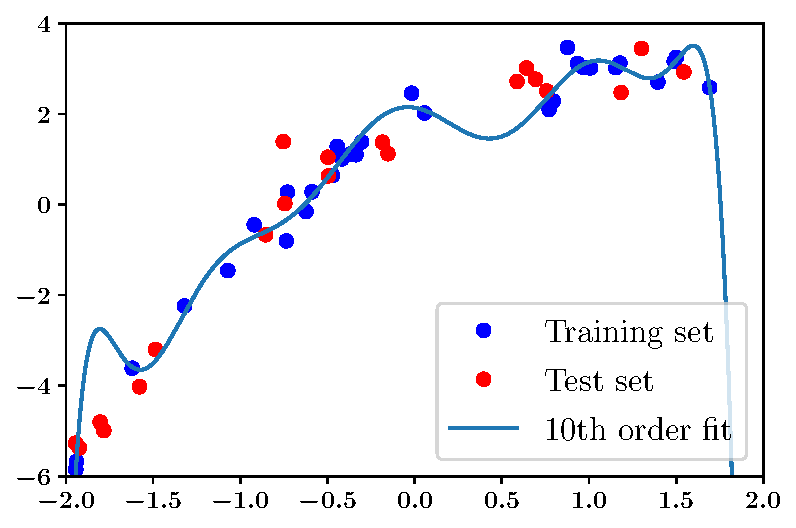
\includegraphics[width=\textwidth]{images/networks/over_under_fit_p10.pdf}
            \label{fig:p10_fit}
        }
    \end{minipage}%
    \hfill%
    \begin{minipage}[c]{0.49\linewidth}
        \vspace{0pt}
        \centering
        \subfloat{
            \begin{tabular}{ccc}
            \toprule
                 & \multicolumn{2}{c}{\textbf{Mean Squared Error}}  \\
            \textbf{Fit order} & \textbf{Train} & \textbf{Test} \\
            \midrule
            1$^\text{st}$ &  1.11 & 1.57 \\
            2$^\text{nd}$ &  0.11 & 0.17 \\
            10$^\text{th}$ &  0.06 & 0.93 \\
            \bottomrule
            \end{tabular}
            \label{tab:fitmse}
        }
    \end{minipage}%
    \caption{Over and underfitting issue in polynomial regression over a set of randomly generated samples. Samples are divided in training set, used for the regression and test set, used to compute the goodness of the fit.
    The fit is performed using a 1$^\text{st}$, 2$^\text{nd}$ and 10$^\text{th}$ degree polynomial, respectively shown in \figref{fig:p1_fit}, \figref{fig:p2_fit} and \figref{fig:p10_fit}. The mean squared error computed over both the training and test set is also reported. }
            \label{fig:overunderfit}
\end{figure}







%\begin{figure}
%    \centering
%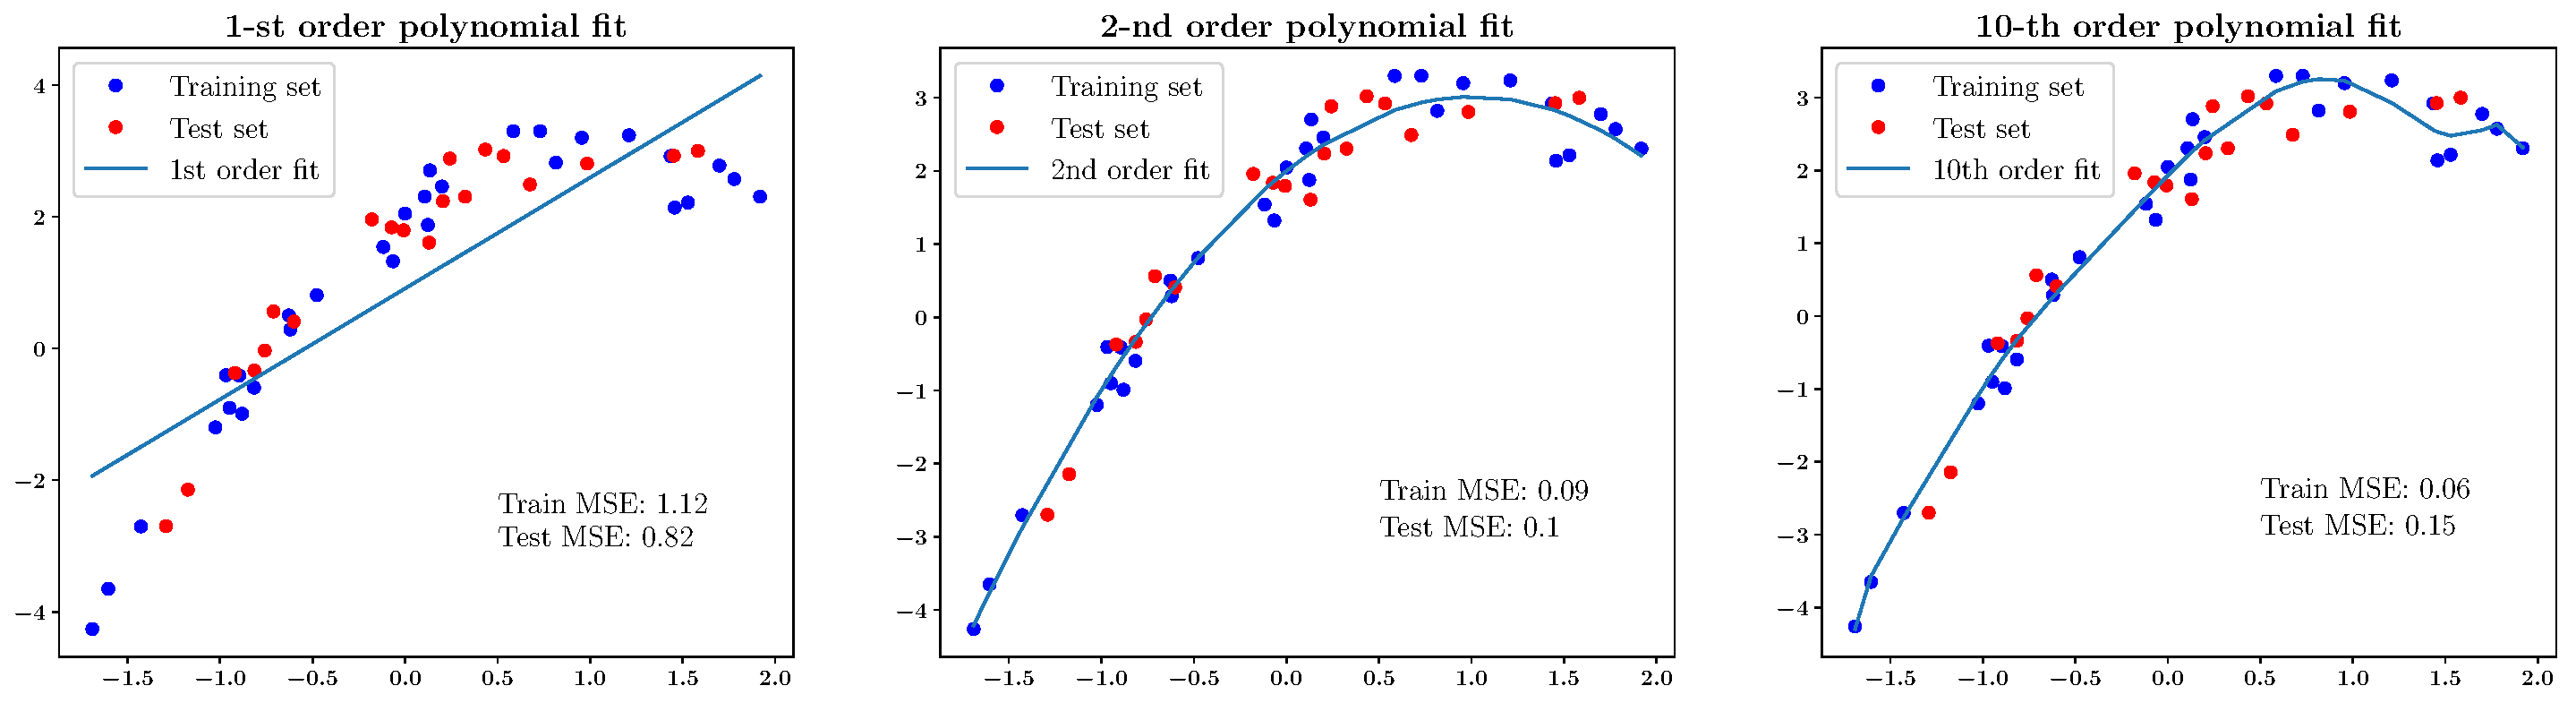
\includegraphics[width=\textwidth]{images/networks/over_under_fit.pdf}
%\caption{overunder fit }
%    \label{fig:overunderfit}
%\end{figure}

\section{Network parameters optimization}\label{weightoptimization}

We have now illustrated the main choices for the creation of an ANN and for the loss function. We know focus on how ann ANN can be trained in order to give relevant prediction respect to the task we are able to solve. 
As we saw in the previous section an ANN is composed by a set of free parameters, namely the weights and biases. The goal of our algorithm is then to find the best parameters able to minimize the value of the selected loss function. This is done using the so-called Backpropagation algorithm, described in \secref{backprop}. This algorithm provides a solid method to compute the gradient of the loss function with respect to the free parameter. The gradient of the loss function is then utilized to update the values of the weights and biases themselves through an optimization algorithm, such as the ones described in \secref{optalg}.
These algorithms are iterated over the full network until a condition, which usually is a maximum number of iterations or a minimum loss value, is met. Each complete iteration of the full gradient estimation and parameter updating is called epoch.

\subsection{Backpropagation algorithm}\label{backprop}

The backpropagation algorithm is divided in two procedures: the Forward propagation and the Back computation.
The Forward propagation corresponds to the computation of the loss function $L(\bar{y}_p, \bar{y}_t)$, where $\bar{y}_p$ is the set of predicted labels, produced by the ANN over an input dataset $\mathcal{D}$, and $\bar{y}_t$ is the set of true labels. 
After the forward propagation is done the backward computation is performed. In this procedure the information from the loss function is propagated backward and used to numerically compute the gradient of the loss function with respect to the free parameters. This allows to easily compute a quantity that would instead take long and difficult analytical computation to be estimated.
More specifically the procedure first computes the gradient of the loss function with respect to each layer and, starting from this values, it estimates the gradient with respect to the single parameter.
The pseudoce of the two procedures is respectively reported  in \algoref{alg:fow_prop} and \algoref{alg:back_comp}, for the forward propagation and backward substitution. 

\begin{algorithm}
\caption{Pseudo-code illustration of the forward propagation procedure for the computation of the predicted labels $\bar{y}_p$ and of the loss function $L(\bar{y}_p,\bar{y}_t)$. In the algorithm the symbol $a^{(i)}$ indicates the activation function of the i-th layer, $f^{(i)}$ its key mathematical operation of the layer and $z^{(i)}$ its output.}
\label{alg:fow_prop}
\begin{algorithmic}[1]
\Require $N_L$ \Comment Depth of the network
\Require $\mathbf{w}^{(i)}$, $i \in \{1,\dots,N_L\}$ \Comment Weight parameters of the network
\Require $b^{(i)}$, $i \in \{1,\dots,N_L\}$ \Comment Bias parameters of the network
\Require $\bar{x}$ \Comment Input value for the prediction
\Require $\bar{y}_t$ \Comment true labels associated to $\bar{x}$

\Procedure{Forward Propagation}{$x$}%\Comment{The g.c.d. of a and b}

\State $z^{(0)} = x$

\For{$k=1,\dots,N_L$} \Comment Loop over the layers
\State $t^{(k)} = b^{(k)} + f^{(k)}\left(\mathbf{w}^{(k)}, z^{(k-1)}\right)$ \Comment Compute operation and apply bias
\State $z^{(k)} = a^{(k)}(t^{(k)})$ \Comment Apply activation function
\EndFor

\State $\bar{y}_p = z^{(N_L)}$

\State \textbf{return} $\hat{y}$, $L(\bar{y}_p,\bar{y}_t)$ \Comment Return predicted labels and loss computation 
\EndProcedure
\end{algorithmic}
\end{algorithm}


\begin{algorithm}
\caption{Pseudo-code illustration of the backward propagation procedure for the computation of the loss gradient respect to each layer. In the algorithm we indicate with $\bar{y}_p$ and $\bar{y}_t$ respectively the set of predicted and true labels. From the \algoref{alg:fow_prop} we use the notation $z^{(k)}$ to indicate the output of a layer and all the values computed in \algoref{alg:fow_prop} are intended as available to the procedure.}
\label{alg:back_comp}
\begin{algorithmic}[1]

\Procedure{Backward Computation}{$x$} \Comment After the forward computation

\State $g \gets \nabla_{\hat{y}}L = \nabla_{\bar{y}_p}L(\bar{y}_p,\bar{y}_t)$\Comment Compute the gradient on the output layer

\For{$k=N_L,N_L-1,\dots,1$}
\State $g \gets \nabla_{t^{(k)}}L = g \odot a^{(k)\prime}(t^{(k)})$
\State $\nabla_{b^{(k)}}L = g$ \Comment Gradient w.r.t biases
\State $\nabla_{\mathbf{w}^{(k)}}L = g z^{(k-1)~T}$ \Comment Gradient w.r.t weight
\State $g \gets \nabla_{z^{(k-1)}}L = \mathbf{w}^{(k)~T} g$ \Comment Gradient w.r.t previous layer
\EndFor

\State \textbf{return} $\nabla_{b^{(k)}}L$, $\nabla_{\mathbf{w}^{(k)}}L$ $\quad$ for $k \in \{1,\dots,N_L\}$ \Comment Return the gradients
\EndProcedure
\end{algorithmic}
\end{algorithm}



\subsection{Optimizers}\label{optalg}

Once the gradient, with respect to each parameter, is computed we can update the parameters themselves. This is done using the so-called optimizers, namely algorithms whose goal is to find the optimal parameters to minimize a function.
For sake of simplicity, in the following we will indicate with $\theta_t$ the value a generic free parameter of the network at the t-th iteration and with $g_{i,t}$ its gradient computed using the i-th sample of the dataset at the t-th iteration.

As for the activation and loss function also the optimizers present multiple choices, one of the most common one is the so-called Mini-batch Gradient Descent (MGD), whose pseudo-code is presented in \algoref{alg:mgd}. This optimizer combines the ideas from two other optimizers: the Grandiet Descent(GD) and Stochastic Gradient Descent (SGD), where both can be derived as an extreme applications of it.

The MGD performs the update of a parameter after computing the gradient over a batch sample, namely a subset of the provided training set, of dimension $n_b$. The choice of the size of this batches greatly influences both speed and stability of the algorithm: bigger batch sizes will in fact result in a more stable convergence at the price of longer computations. Once the gradient is computed the parameters are updated using the following rule:
\begin{equation}
\theta_{t+1}=\theta_t-\eta \cdot \sum_{i=1}^{n_b} g_{i,t}
\end{equation}

where $\eta$ is a parameter called learning rate which quantifies the "speed" at which the update procedure is performed\footnote{The choice of $\eta$ can also greatly influences the convergence of the algorithm: too small values will result in slower algorithms and also present the risk of the algorithm remaining stuck in local minimums but, on the other hand, a value too high of the learning rate may lead to an unstable algorithm.}. 

The two extreme cases for this algorithm are the choice of performing the update for each sample in the training set, in which case we have the SGD algorithm, or performing the update after computing the gradient over the whole dataset, which correspond to the GD algorithm. 

Another really popular and powerful choice for the optimization algorithm is the so-called Adaptive Moment Estimation optimizer, better known as ADAM. This optimizer belong, as the name suggests, to the group of adaptive optimizers. Optimizers of this group instead of using a fixed learning rate $\eta$, as in the MGD case, adapt the learning rate to each parameters.
The power of this type of methods lies in its ability to adjust the amount of update a specific parameter receives, based on both the importance and the frequency of the features connected to it. 

To do this the ADAM optimizer, whose pseudo-code is illustrated in \algoref{alg:adam}, uses the information on the gradients over the past iterations of the algorithm, while introducing three new parameter $\beta_1$, $\beta_2$ and $\epsilon$. As before the gradient can be computed over batches of different sizes but, for simplicity, we will indicate with $g_t$ the gradient computed over a mini-batch of arbitrary size. The first step of the algorithm is the computation of the following quantities:
\begin{equation}
\begin{aligned}
m_{t} &=\beta_{1} m_{t-1}+\left(1-\beta_{1}\right) g_{t} \\
v_{t} &=\beta_{2} v_{t-1}+\left(1-\beta_{2}\right) g_{t}^{2}
\end{aligned}
\end{equation}

The $m_t$ and $v_t$ are respectively an estimation of the first and second momentum of the past gradient, namely the mean and not centered variance. The suggested values for the $\beta$ parameters are respectively $\beta_1=0.9$ and $\beta_2=0.999$. As observed by the original authors, the $m_t$ and $v_t$ values are however biased toward zero, due to them being initially set to a null value. To solve this problem they are scaled as:
\begin{equation}
\begin{aligned}
\hat{m}_{t} &=\frac{m_{t}}{1-\beta_{1}^{t}} \\
\hat{v}_{t} &=\frac{v_{t}}{1-\beta_{2}^{t}}
\end{aligned}
\end{equation}

This values are now used to computed the update of the free parameter $\theta$ with the following rule:
\begin{equation}
\theta_{t+1}=\theta_{t}-\frac{\eta}{\sqrt{\hat{v}_{t}}+\epsilon} \hat{m}_{t}
\end{equation}

where $\eta$ is the generic learning rate and the suggested value for the $\epsilon$ variable is $\epsilon=10^{-8}$. It is also empirically shown that the ADAM algorithm is works really well with favorable results in the comparison to other algorithms of this type.

\begin{algorithm}[H]
\caption{Pseudo-code illustration of the updating procedure of a free parameter $\theta$ using the Mini-batch Gradient Descent (MGD) algorithm. In the following N represents the total number of elements in the full dataset. We also indicate with $x^{(i)}$ and $y^{(i)}_t$ the i-th sample of the dataset and its corresponding label and with $g_{i,t}$ the gradient computed using the i-th sample with respect to the parameter $\theta$ at the iteration t. }
\label{alg:mgd}
\begin{algorithmic}[1]
\Require $\eta$ \Comment Learning rate
\Require ${\theta}$ \Comment Initial free parameter
\Require $n_b$\Comment Minibatch dimension 

\Procedure{MGD}{$\{x^{(i)}\}_{i=1,\dots,N}$} 
\While{Stop condition is False} \Comment Loop until an exit condition is met
\State $\bar{x}_b \gets \{x^{(1)},\dots,x^{(m)}\}$\Comment Sample a minibatch
\State $\bar{y}_b \gets \{y^{(1)_t},\dots,y^{(m)_t}\}$\Comment Sample label corresponding to the minibatch
\State ${g}_t \gets  \frac{1}{m} \sum_{i=1}^{n_b} g_{t,i}$ \Comment{Compute gradient over minibatch}
\State $\theta_{t+1} \gets \theta_t - \eta\cdot {g}_t$ \Comment Update parameter
\EndWhile

\State \textbf{return} ${\theta}$
\EndProcedure
\end{algorithmic}
\end{algorithm}




\begin{algorithm}[H]
\caption{Pseudo-code illustration of the updating procedure of a free parameter $\theta$ using the Adaptive Moment Estimation (ADAM) algorithm. In the following N represents the total number of elements in the full dataset. We also indicate with $x^{(i)}$ and $y^{(i)}_t$ the i-th sample of the dataset and its corresponding label and with $g_{i,t}$ the gradient computed using the i-th sample with respect to the parameter $\theta$ at the iteration t. Suggested values for the parameters of are $\beta_1=0.9,\,\beta_2=0.999,\,\epsilon=10^{-8}$}\label{alg:adam}
\begin{algorithmic}[1]
\Require $\eta ,\, \beta_1,\,\beta_2,\,\epsilon$ \Comment Algorithm parameters and learning rate
\Require ${\theta}$ \Comment Initial free parameter
\Require $n_b$\Comment Minibatch dimension 

\Procedure{ADAM}{$\{x^{(i)}\}_{i=1,\dots,n}$} 
\State $s\gets 0;\quad r\gets 0$ \Comment Initialize $1^\text{st}$ and $2^\text{nd}$ momentum 
\State $k\gets 0$ \Comment Initialize and iteration counter

\While{Stop condition is False} \Comment Loop until an exit condition is met

\State $\bar{x}_b \gets \{x^{(1)},\dots,x^{(m)}\}$\Comment Sample a minibatch
\State $\bar{y}_b \gets \{y^{(1)_t},\dots,y^{(m)_t}\}$\Comment Sample label corresponding to the minibatch
\State ${g}_t \gets  \frac{1}{m} \sum_{i=1}^{n_b} g_{t,i}$ \Comment{Compute gradient over minibatch}

\State $k \gets k+1$
\State $m_t \gets \beta_1 m_{t-1} + (1-\beta_1) g_t$    \Comment Compute first momentum
\State $v_t \gets \beta_2 v_t + (1-\beta_2) g_t \cdot g_t$    \Comment Compute second momentum
\State $\hat{m_t} \gets \frac{m_t}{1 - \beta^k_1}$   \Comment Correct bias in first momentum
\State $\hat{v_t} \gets \frac{v_t}{1 - \beta^k_2}$   \Comment Correct bias in second momentum
\State $\theta_{t+1}=\theta_{t}-\frac{\eta}{\sqrt{\hat{v}_{t}}+\epsilon} \hat{m}_{t}$
\Comment Perform Parameter update
\EndWhile

\State \textbf{return} ${\theta}$
\EndProcedure
\end{algorithmic}
\end{algorithm}

\section{Additional optimization techniques} \label{opt_tec}

When the an ANN architecture reaches an high number of parameters and/or  presents really deep or complex architectures it is necessary to implement some other optimization techniques, in order for it to be able to solve the designated task. In this section we will focus on the two mostly implemented techniques, which are used in most of the common application.

\subsection{Regularization}\label{regularization}

Regularization is one of the central topics is the Machine Learning framework. Its goal is to reduce the generalized error, namely the error on a test set, while not modifying the error on the training set. The regularization topic is directly connected to the overfitting issue, described in the previous section and is in fact one of the most robust ways to prevent it. 

The regularization is implemented defining a new regularized loss function, obtained by adding an additional term to the original loss function. Indicating with $L(\boldsymbol{w},\bar{b})$ the loss function and its depence on the weight and biases of the network, we define the regularized loss function $J(\mathbf{w}, \vec{b})$ as:
\begin{equation}
J(\mathbf{w}, \vec{b})=L(\mathbf{w}, \vec{b})+ \lambda\Omega(\mathbf{w})
\end{equation}

where $\lambda$ is a parameter that regulates the importance of the regularization respect to the loss and the $\Omega(\mathbf{w})$ is a function depending on the weights of the network. 

The choices for the $\Omega(\mathbf{w})$ function are mainly restricted to two alternatives:
\begin{itemize}
    \item \textbf{L1 regularization}: $\Omega_{L1}(\mathbf{w}) = \sum_{i=1}^N |w_i|$
    \item \textbf{L2 regularization}: $\Omega_{L2}(\mathbf{w}) = \sum_{i=1}^N w_i^2$
\end{itemize}

The main difference between the two is the macroscopic effect obtained after their implementation. The L1 regularization in fact tends to reduce the number of features that influences the final prediction while the L2 regularization reduces the influence that each feature has on it.


\subsection{Dropout}\label{dropout}

Another popular technique, often implemented to avoid overfitting, is the so-called dropout. The concept behind this technique is rather simple: given the hyperparameter\footnote{Hyperparameters are parameters of the network estimated before the start of the training and kept fixed during the whole procedure. Example of other hyperparameters are the learning rate of the optimizers and parameter $\lambda$ for the regularization.} $\rho\in [0,1]$, called "dropout rate", at each training epoch each neuron has a probability $\rho$ of being stopped. A stopped neuron is completely ignored and not updated during the entire iteration.
An illustation of the implementation of the dropout is shown in \figref{fig:dropout}. The effectiveness of this method can be explained by considering the effect it has on the single neurons. When the dropout is implemented there is in fact less possibility for neighbour neurons to co-adapt in order to give a good prediction, resulting in an improved performance of the single units and in a more robust ANN as a whole.

\begin{figure}
    \centering
\includestandalone[width=\textwidth]{images/networks/dropout}
\caption{Example of the implementation of the dropout technique in a fully connected ANN model. The single neurons that are excluded after the dropout are indicated with crossed circles and their connection removed. }
    \label{fig:dropout}
\end{figure}



